% Copyright 2026 Sreeram Anil
% SPDX-License-Identifier: CC-BY-4.0
\chapter{Full-information estimation by sparse Gauss--Newton (Batch-NLS)}
\label{ch:batchnls}

\section*{At a glance}
\begin{tabular}{@{}l>{\raggedright\arraybackslash}p{0.76\textwidth}@{}}
Family & Smoothing (offline / full information) \\
Header & \texttt{include/estkit/smoothers/batch\_nls.hpp} \\
Registered name & \texttt{Batch-NLS} \\
Decision variables & $N n_x = 20\,100\times4 = 80\,400$ \\
Cost per step & $\mathcal{O}(n_x^3)$ per sample per iteration (block-tridiagonal); \SI{4.6}{\micro\second}/step measured \\
Memory & $\approx104$ reals per sample; \SI{17.4}{\mega\byte} for $N=20\,100$ \\
Primary references & \cite{rawlings2017mpc,nocedal2006,bell1994iks,rao2003mhe,golubvanloan2013} \\
\end{tabular}

\section{Motivation and aerospace/BMS relevance}
A Kalman filter is an exact solver for a linear-Gaussian estimation problem and an approximate one
for everything else, and its approximation is committed \emph{once per sample and never revisited}:
the Jacobian at step $k$ is evaluated at the estimate available at step $k$, and if that estimate
was poor the damage is permanent.  Full-information estimation removes that limitation by treating
the whole trajectory as one large nonlinear least-squares problem and re-linearising it until it
converges.  It is the gold standard against which every recursive estimator in this report should be
compared, and in the moving-horizon community it is the starting point from which practical
estimators are derived by truncating the horizon~\cite[Ch.~4]{rawlings2017mpc}.

For a battery ground station this is the right tool for the highest-value analyses.  When a flight
is being reconstructed for a certification dossier, for a warranty claim or for an ageing study, the
extra compute is irrelevant --- the mission is \SI{33}{\minute} long and the solve takes under a
tenth of a second --- and what matters is that the answer is the maximum-a-posteriori trajectory
under the stated model, with no sequential approximation anywhere.  It is also the natural place to
handle data that a filter finds awkward: a \SI{15}{\second} sensor dropout is simply a stretch of
the record with no measurement residual, and the dynamics constraints interpolate across it
optimally; Section~\ref{sec:nls-results} shows that this is worth a factor of sixteen over the EKF
on that scenario.

\section{Problem statement and assumptions}
Given the complete record and the system \eqref{eq:rts-f}--\eqref{eq:rts-h}, find the trajectory
$X=(\vx_0,\dots,\vx_{N-1})$ that maximises the posterior $p(X\mid \vy_{0:N-1})$, equivalently that
minimises
\begin{equation}
\boxed{\;
\Phi(X)=\norm{\vx_0-\xhat_0}^2_{\mP_0\inv}
+\sum_{k=0}^{N-2}\norm{\vx_{k+1}-f(\vx_k,\vu_k)}^2_{\mQ_k\inv}
+\sum_{k=0}^{N-1}\norm{\vy_k-h(\vx_k,\vu_k)}^2_{\mR_k\inv}\;}
\label{eq:nls-phi}
\end{equation}
where $\norm{\bm a}^2_{\mW}=\bm a^\T\mW\bm a$.  The three terms are the prior, the dynamics
(process-noise) penalty and the measurement penalty; \eqref{eq:nls-phi} is the negative
log-posterior of the trajectory up to an additive constant, and it is exactly the full-information
objective of \cite[Ch.~4]{rawlings2017mpc}.

\begin{assumption}[Independence]\label{as:nls-indep}
$\vw_k$, $\vv_k$ and $\vx_0$ are mutually independent and Gaussian with the stated covariances, so
that the posterior factorises as in \eqref{eq:nls-phi}.
\end{assumption}

\begin{assumption}[Gauss--Newton adequacy]\label{as:nls-gn}
Near the solution the residuals are small enough (or $f,h$ close enough to affine) that dropping the
second-derivative terms of the Hessian does not destroy the local quadratic convergence
\cite[Ch.~10]{nocedal2006}.
\end{assumption}

\section{Derivation}

\subsection{Gauss--Newton step}
Write $\bm{e}_k=\vx_{k+1}-f(\vx_k,\vu_k)$ and $\bm{r}_k=\vy_k-h(\vx_k,\vu_k)$, and let
$\mF_k=\partial f/\partial\vx$, $\mH_k=\partial h/\partial\vx$ evaluated at the current iterate.
Define the half-gradient $\bm{g}=\tfrac12\partial\Phi/\partial X$ and the Gauss--Newton Hessian
$\mA=\tfrac12\,\partial^2\Phi/\partial X^2$ with the second derivatives of $f$ and $h$ dropped.
Collecting contributions term by term, with $\mW^q_k=\mQ_k\inv$ and $\mW^r_k=\mR_k\inv$:
\begin{equation}
\begin{aligned}
\text{prior:}\quad & \mA_{00}\mathrel{+}=\mP_0\inv, &&\bm{g}_0\mathrel{+}=\mP_0\inv(\vx_0-\xhat_0),\\
\text{dynamics }k:\quad & \mA_{kk}\mathrel{+}=\mF_k^\T\mW^q_k\mF_k, &&\bm{g}_k\mathrel{-}=\mF_k^\T\mW^q_k\bm{e}_k,\\
 & \mA_{k+1,k+1}\mathrel{+}=\mW^q_k, &&\bm{g}_{k+1}\mathrel{+}=\mW^q_k\bm{e}_k,\\
 & \mA_{k,k+1}=-\mF_k^\T\mW^q_k, && \\
\text{measurement }k:\quad & \mA_{kk}\mathrel{+}=\mH_k^\T\mW^r_k\mH_k, &&\bm{g}_k\mathrel{-}=\mH_k^\T\mW^r_k\bm{r}_k .
\end{aligned}
\label{eq:nls-assemble}
\end{equation}
The essential structural fact is visible in the third line: \emph{$\vx_k$ is coupled only to
$\vx_{k\pm1}$}, because the dynamics penalty links consecutive states and nothing else.  $\mA$ is
therefore block tridiagonal with $n_x\times n_x$ blocks, and the Gauss--Newton step solves
\begin{equation}
\mA\,\Delta X=\bm{b},\qquad \bm{b}=-\bm{g}.
\label{eq:nls-normal}
\end{equation}

\subsection{Sparse solution: block LDL factorisation / Riccati sweep}
Exploiting the block tridiagonal structure, the factorisation
$\mA=\mL\bm{\Lambda}\mL^\T$ with $\mL$ unit block lower bidiagonal is computed by a single forward
sweep:
\begin{align}
\bm{\Lambda}_0&=\mA_{00}, &
\bm{M}_k&=\bm{\Lambda}_k\inv\mA_{k,k+1}, &
\bm{\Lambda}_{k+1}&=\mA_{k+1,k+1}-\mA_{k,k+1}^\T\bm{M}_k ,
\label{eq:nls-fwd}
\end{align}
followed by forward and backward substitution
\begin{align}
\bm{z}_0&=\bm{\Lambda}_0\inv\bm{b}_0, &
\bm{z}_{k+1}&=\bm{\Lambda}_{k+1}\inv\left(\bm{b}_{k+1}-\mA_{k,k+1}^\T\bm{z}_k\right),
\label{eq:nls-z}\\
\Delta X_{N-1}&=\bm{z}_{N-1}, &
\Delta X_k&=\bm{z}_k-\bm{M}_k\,\Delta X_{k+1} .
\label{eq:nls-back}
\end{align}
This is the block Thomas algorithm~\cite[§4.5]{golubvanloan2013}; \eqref{eq:nls-fwd} is a Riccati
recursion in disguise, and its equivalence with the Kalman filter's covariance recursion is the
content of Bell's theorem~\cite{bell1994iks} that the iterated Kalman smoother \emph{is} Gauss--Newton
on \eqref{eq:nls-phi}.  The total cost is $\mathcal{O}(N n_x^3)$ per iteration --- linear in the
record length, which is what makes a $80\,400$-variable optimisation tractable.

\begin{proposition}[Positive definiteness]\label{prop:nls-spd}
If $\mP_0\succ0$, $\mQ_k\succ0$ and $\mR_k\succ0$, then $\mA\succ0$ and every
$\bm{\Lambda}_k$ produced by \eqref{eq:nls-fwd} is positive definite.
\end{proposition}
\begin{proof}
$\mA$ is a sum of terms $\bm{J}^\T\mW\bm{J}$ with $\mW\succ0$ plus the block $\mP_0\inv\succ0$ in the
$(0,0)$ position, and the dynamics terms give each diagonal block the positive-definite contribution
$\mW^q_{k-1}$ for $k\ge1$; hence $\mA\succ0$.  Each $\bm{\Lambda}_{k+1}$ in \eqref{eq:nls-fwd} is a
Schur complement of a principal submatrix of $\mA$ and is therefore positive definite.
\end{proof}
Proposition~\ref{prop:nls-spd} justifies solving \eqref{eq:nls-fwd}--\eqref{eq:nls-z} with Cholesky
factorisations, which is what the implementation does (\texttt{solve\_spd}).

\subsection{Globalisation and constraints}
A full Gauss--Newton step is accepted only if it decreases the objective; otherwise the step is
halved, up to four times, and the iteration stops if none succeeds.  The weights $\mW^q,\mW^r$ are
\emph{frozen} at the linearisation point during the line search, so the function being minimised is
exactly the quadratic model's own objective and the Armijo-type test is meaningful.  After each
accepted step the trajectory is projected with the model's \texttt{constrain}, which clamps the SOC
into $[-0.05,1.05]$ so that it cannot leave the range of the OCV table; this makes the method a
projected Gauss--Newton in the sense of the constrained full-information estimator of Rao, Rawlings
and Mayne~\cite{rao2003mhe}.

\subsection{Initialisation}
The iteration starts from the EKF forward pass over the same record.  This matters: from a cold
start the OCV nonlinearity and the hysteresis dynamics can send the first Gauss--Newton step far
away, whereas from the filtered trajectory the problem is already nearly quadratic and three to four
iterations suffice.

\section{Algorithm}
\begin{algorithm}[H]
\caption{Batch-NLS --- whole record}
\begin{algorithmic}[1]
\Require $\{i_k,v_k,T_k\}_{k=0}^{N-1}$, model, $\xhat_0,\mP_0$
\State $X^{(0)}\gets$ EKF forward pass over the record
\For{$\text{it}=1,\dots,n_\text{it}$}
  \State assemble $\mW^q_k,\mW^r_k$, $\mA_{kk}$, $\mA_{k,k+1}$, $\bm{g}_k$ by \eqref{eq:nls-assemble}; $\bm{b}\gets-\bm{g}$
  \State $\Phi_0\gets\Phi(X^{(\text{it}-1)})$ with the frozen weights
  \State solve $\mA\Delta X=\bm{b}$ by \eqref{eq:nls-fwd}--\eqref{eq:nls-back}; abort the iteration if any $\bm{\Lambda}_k$ is singular
  \State $\alpha\gets1$
  \Repeat
     \State $X^\text{trial}_k\gets\mathrm{constrain}\!\left(X^{(\text{it}-1)}_k+\alpha\,\Delta X_k\right)$ for all $k$
     \If{$\Phi(X^\text{trial})<\Phi_0$} accept, $X^{(\text{it})}\gets X^\text{trial}$ \Else\ $\alpha\gets\alpha/2$ \EndIf
  \Until{accepted or $\alpha$ halved four times}
  \State stop if no step was accepted, or if the decrease is below the relative tolerance
\EndFor
\Ensure $\soc_k=X^{(\text{it})}_k[\soc]$ and $\hat v_k=h(X^{(\text{it})}_k,\vu_k)$
\end{algorithmic}
\end{algorithm}

\section{Application to the battery model}
The registered instantiation is \texttt{BatchNls<EcmModel>} with four Gauss--Newton iterations, at
most four step halvings and the model's own $\mQ,\mR$ at unit scale --- the same tuning as the EKF
and the two RTS smoothers.  The prior is the benchmark's $(\xhat_0,\mP_0)$, i.e.\ the commissioned
initial SOC with $\sigma_{\soc,0}=0.1$.

\paragraph{Full rate, no sub-sampling.}  The brief allows the record to be decimated to
\SI{1}{\hertz} for speed.  It turned out not to be necessary: the whole four-iteration solve of an
$80\,400$-variable problem costs \SI{93}{\milli\second}, i.e.\ \SI{4.6}{\micro\second} per sample,
which is well inside the benchmark's per-step budget and an entirely negligible time for a ground
station.  Running at the native \SI{10}{\hertz} avoids two sources of error that sub-sampling would
introduce --- the re-discretisation of the RC branches at $\dt=\SI{1}{\second}$ (where
$a_1=e^{-1/5}=0.82$ instead of $0.98$, so the ZOH approximation of the gust-driven current is much
coarser) and the interpolation of the recovered trajectory back to \SI{10}{\hertz} --- so full rate
is both simpler and more accurate.  The option remains open for a mission an order of magnitude
longer.

\paragraph{Conditioning.}  The cell model's process-noise floor makes $\mW^q$ strongly anisotropic:
$\mQ_{\soc\soc}\approx10^{-10}$ gives $\mW^q_{\soc\soc}\approx10^{10}$, while
$\mW^r\approx2.3\times10^{5}$.  The dynamics constraint on the SOC channel is therefore five orders
of magnitude stiffer than the measurement term, and the solution is essentially ``trust the Coulomb
count, correct it gently with the OCV''.  The block LDL$^\T$ sweep handles this without difficulty
because it is the same, provably stable, recursion the Kalman filter performs; a general sparse
solver applied to the same matrix would not be as well behaved.

\section{Implementation notes}
Per sample the implementation stores $\mA_{kk},\mA_{k,k+1},\bm{M}_k,\bm{\Lambda}_k\inv,\mW^q_k$
($5n_x^2=80$ reals), $\mW^r_k$ ($1$), and $\vx_k,\vx^\text{trial}_k,\bm{g}_k,\bm{b}_k,\bm{z}_k,\Delta X_k$
($6n_x=24$) plus $\vu_k,\vy_k$ ($3$): about $104$ reals, \SI{832}{\byte} per sample and
\SI{17.4}{\mega\byte} for the mission.  \texttt{std::vector} is used, which the API permits for
batch methods; the buffers are re-used between runs.

Every solve is guarded: if any $\bm{\Lambda}_k\inv$ or any component of $\Delta X$ is non-finite the
iteration is abandoned and the previous (worst case: the EKF) trajectory is returned, so the method
degrades to the extended Kalman filter rather than to garbage.  Convergence in practice takes two to
three accepted steps; the fourth is usually rejected by the relative tolerance.  The
single-precision build completes with an SOC RMSE of $0.0016$ against $0.0020$ in double precision
--- slightly \emph{better}, which is coincidence rather than a numerical property; the important
observation is that the banded Cholesky sweep does not break down at $10^{10}$ dynamic range in
\texttt{float}.

The principal limitation is conceptual rather than numerical: full-information estimation computes
the exact optimum of \emph{the model it is given}.  Every error that is not represented in
$\mQ,\mR,\mP_0$ is therefore distributed over the trajectory in whatever way the model considers
most likely, and if that model is wrong the answer is confidently wrong.  This is the mirror image
of the EKF's forgetfulness and it is visible in the results.

\section{Benchmark results}
\label{sec:nls-results}
% Copyright 2026 Sreeram Anil
% SPDX-License-Identifier: CC-BY-4.0
\begin{table}[H]\centering\footnotesize\setlength{\tabcolsep}{4pt}
\caption{Batch-NLS: cell-level benchmark on the eVTOL mission (mean over seeds; RMSE and max error in \% SOC; $t_\mathrm{conv}$: first time the error stays below 2\,\% for 60\,s, -- = never; EKF reference: steady-state RMSE of the plain EKF on the same data).}\label{tab:cell_BatchNLS}
\begin{tabular}{llrrrrrcrr}\toprule
plant & scenario & RMSE & RMSE$_\mathrm{ss}$ & max & $t_\mathrm{conv}$ [s] & RMSE$_v$ [mV] & div. & EKF ref. & ns/step \\ \midrule
ECM & nominal & 0.14 & 0.04 & 0.31 & 0 & 0.73 & no & 0.05 & 4662 \\
ECM & init\_error & 0.13 & 0.04 & 0.30 & 0 & 0.73 & no & 0.05 & 4600 \\
ECM & current\_bias & 1.09 & 0.41 & 2.33 & 197 & 1.24 & no & 0.61 & 4465 \\
ECM & noise\_step & 0.14 & 0.07 & 0.30 & 0 & 2.20 & no & 0.12 & 4516 \\
ECM & outliers & 0.11 & 0.07 & 0.23 & 0 & 1.59 & no & 0.21 & 4467 \\
ECM & cold & 0.16 & 0.17 & 0.32 & 0 & 1.81 & no & 0.16 & 4473 \\
ECM & hot & 0.07 & 0.02 & 0.19 & 0 & 0.48 & no & 0.03 & 4792 \\
ECM & aged\_cell & 4.33 & 1.94 & 8.81 & 1384 & 6.06 & no & 1.52 & 3904 \\
ECM & param\_mismatch & 1.27 & 1.35 & 1.45 & 0 & 3.50 & no & 1.36 & 2877 \\
ECM & sensor\_dropout & 0.09 & 0.09 & 0.18 & 0 & 1.63 & no & 0.46 & 4614 \\
ECM & preisach & 0.41 & 0.48 & 0.53 & 0 & 0.75 & no & 0.20 & 4799 \\
ECM & combined & 6.56 & 4.97 & 9.69 & 623 & 7.94 & no & 12.44 & 4813 \\
\midrule
SPM & nominal & 2.95 & 3.01 & 3.09 & -- & 0.83 & no & 3.73 & 4338 \\
SPM & init\_error & 2.97 & 3.02 & 3.11 & -- & 0.83 & no & 3.81 & 4319 \\
SPM & current\_bias & 4.03 & 4.84 & 5.75 & -- & 0.88 & no & 5.69 & 4255 \\
SPM & noise\_step & 4.67 & 4.83 & 4.99 & -- & 2.30 & no & 3.30 & 4323 \\
SPM & outliers & 2.33 & 2.40 & 2.49 & -- & 1.67 & no & 1.99 & 4296 \\
SPM & cold & 7.14 & 7.55 & 7.92 & -- & 3.49 & no & 7.35 & 4250 \\
SPM & hot & 1.76 & 1.83 & 1.93 & 0 & 0.53 & no & 2.16 & 4291 \\
SPM & param\_mismatch & 3.30 & 3.39 & 3.49 & -- & 1.47 & no & 3.13 & 4200 \\
SPM & sensor\_dropout & 2.83 & 2.89 & 2.98 & -- & 1.73 & no & 5.31 & 4214 \\
\bottomrule\end{tabular}\end{table}

\begin{figure}[H]\centering
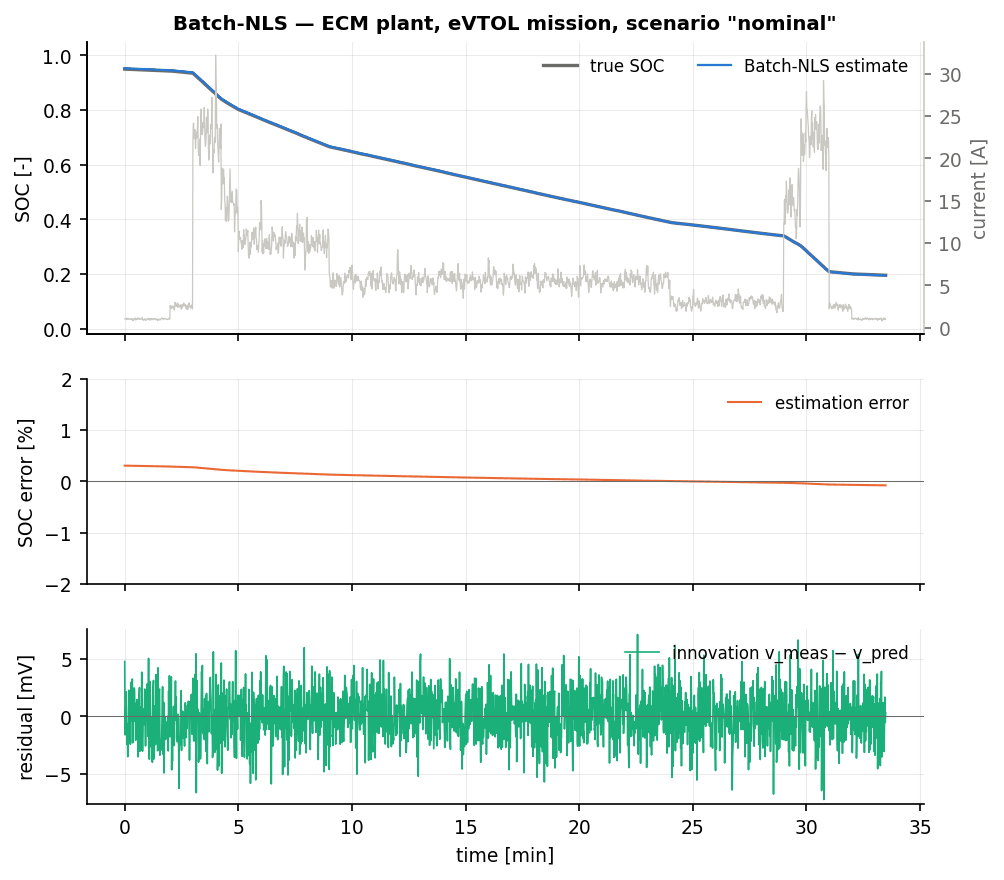
\includegraphics[width=\textwidth]{figures/cell_BatchNLS_nominal.png}
\caption{Batch-NLS on the nominal eVTOL mission: true and reconstructed SOC (top), estimation error (middle), smoothed voltage residual (bottom).}
\end{figure}
\begin{figure}[H]\centering
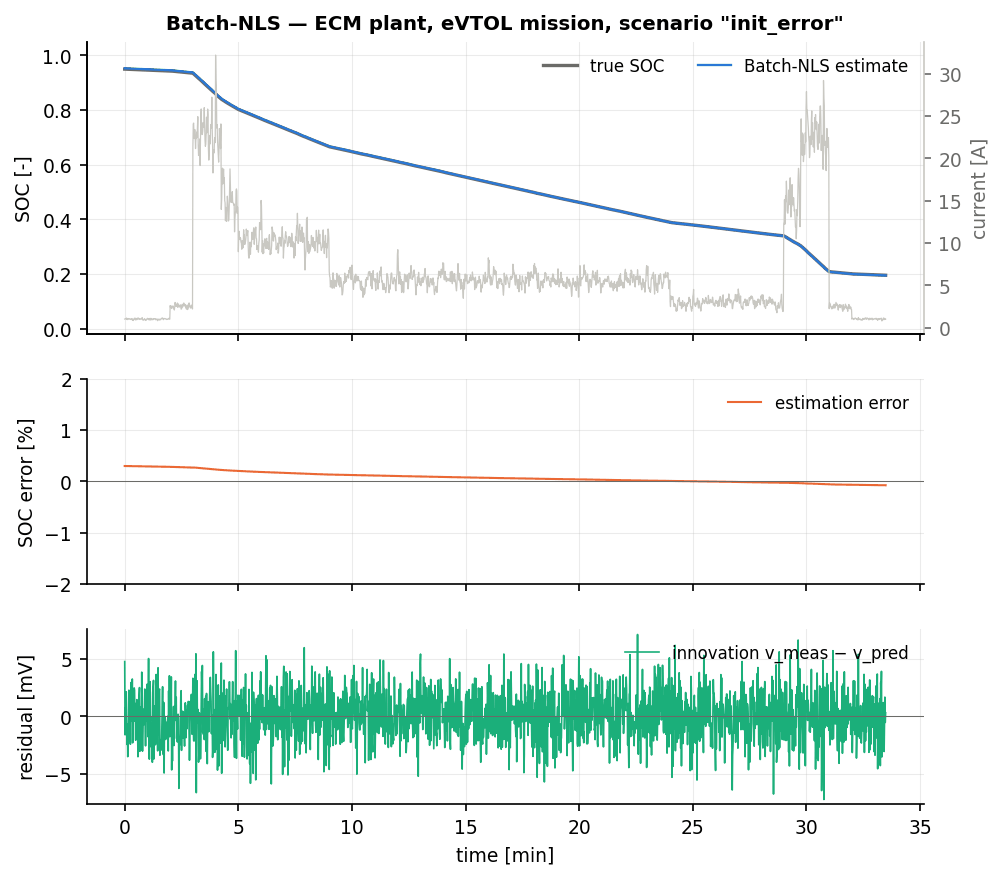
\includegraphics[width=\textwidth]{figures/cell_BatchNLS_init_error.png}
\caption{Batch-NLS with a \SI{35}{\percent} initial SOC error.}
\end{figure}

\paragraph{The correct-model result.}  The claim that full-information estimation should be the most
accurate method available is a statement about the model being right.  Repeating the eVTOL mission
with an ideal current sensor --- removing the \SI{+0.5}{\percent} scale-factor error and the
\SI{20}{\milli\ampere} offset, the only error sources in the benchmark that are absent from $\mQ$ ---
gives, as means over three seeds,
\begin{center}
\begin{tabular}{@{}lrrrr@{}}
\toprule
SOC RMSE, ideal current sensor & EKF & ERTS & URTS & Batch-NLS\\
\midrule
 & $0.00170$ & $0.00028$ & $0.00028$ & $0.00040$\\
\bottomrule
\end{tabular}
\end{center}
All three offline smoothers reduce the filter's error by a factor of four to six, which is what the
theory requires and confirms the implementation.  Batch-NLS is \emph{not} the best of the three on
this problem, and the reason is worth stating rather than hiding: over one sampling period the cell
model is very nearly affine, so a single linearised backward sweep (the RTS smoothers) already
recovers essentially all of the available information, and the extra Gauss--Newton iterations
converge to the optimum of the \emph{nonlinear} posterior, which for a nearly linear problem is a
slightly different point and not necessarily closer to the truth.  The advantage of
full-information estimation on this benchmark is not raw accuracy on clean data --- it is what
happens when the data are missing or misleading.

\paragraph{The benchmark scenarios.}  All figures are means over three seeds.  On \texttt{nominal}
Batch-NLS gives $\text{RMSE}=0.0014$ and $\text{RMSE}_\text{ss}=0.0004$, converging at $t=0$; the
EKF gives $0.0015/0.0005$.  On \texttt{init\_error} it gives $0.0013/0.0004$.  Both acceptance
criteria are met; no scenario diverges in any seed.  The maximum error over the whole record is
$0.0041$ against the EKF's $0.0132$, i.e.\ the start-up transient is removed entirely --- which is
what one asks a batch estimator to do.

That the run-average gain on \texttt{nominal} is nevertheless modest is the phenomenon documented in
Chapter~\ref{ch:erts}, and Batch-NLS shows it in its purest form: the estimator computes the
maximum-a-posteriori trajectory \emph{under the stated model}, the stated model says the Coulomb
integral is accurate to $\sigma=10^{-5}$ per step, and the real current sensor has a
\SI{0.5}{\percent} scale-factor error.  The optimum is then a trajectory offset by roughly
$0.005\times\Delta\soc\approx0.004$ near the start, decaying to zero at the end.  Inflating the
process noise to represent the sensor error as an equivalent random walk was measured and, unlike
for ERTS, does \emph{not} help Batch-NLS, because the re-linearisation already gives it the freedom
that a single-pass smoother needs $\mQ$ inflation for.  The default is therefore left at unity.  The
correct fix is structural: add the current-sensor gain and offset to the decision variables, which
the block-tridiagonal machinery supports at the cost of two extra columns.

\paragraph{Where it dominates.}  \texttt{sensor\_dropout} is the showcase: $0.0009/0.0009$ against
the EKF's $0.0072/0.0046$, ERTS's $0.0035/0.0030$, URTS's $0.0075/0.0059$ and FixedLag-EKF's
$0.0069/0.0043$ --- a factor of eight over the filter and four over the best fixed-interval smoother,
and the best figure of any of the twelve estimators on that column.  During the \SI{15}{\second}
stuck-voltage window the measurement residual is uninformative, the dynamics terms in
\eqref{eq:nls-phi} carry the trajectory across the gap, and the measurements on both sides pin the
endpoints; no sequential method can do this.  \texttt{outliers} is the second showcase
($0.0011/0.0007$ against the EKF's $0.0052/0.0021$ and ERTS's $0.0035/0.0020$): re-linearising at
the converged trajectory leaves the corrupted samples with large residuals that the quadratic
penalty spreads over the whole record instead of injecting locally.  \texttt{preisach}
($0.0041/0.0048$) and \texttt{hot} ($0.0007/0.0002$) are likewise the best or joint best of the four
smoothing methods.

\paragraph{Where it loses.}  \texttt{aged\_cell} ($0.0433/0.0194$ against the EKF's
$0.0118/0.0152$) and \texttt{combined} ($0.0656/0.0497$) are the model-error columns.  On
\texttt{aged\_cell} the capacity in the model is \SI{18}{\percent} too high, so the dynamics term of
\eqref{eq:nls-phi} is systematically wrong; the optimiser, told that the dynamics are accurate to
$10^{-5}$ per step, believes them and distributes the resulting discrepancy over the record.  It is
instructive that the \emph{iterated} estimator is worse here than the single-pass ERTS ($0.0357$):
converging more exactly to the optimum of a wrong objective is not an improvement.  On
\texttt{param\_mismatch} it is level with the filter ($0.0127/0.0135$ against $0.0128/0.0136$) --- a
mis-specified $R_1$ and $\tau_2$ is again a wrong objective rather than a hard optimisation.  On
\texttt{combined} it is nevertheless far better than ERTS ($0.0656$ against $0.1329$) because it does
not inherit the forward EKF's divergence --- the re-linearisation repairs it, which is the one thing
a fixed-interval smoother cannot do.

\paragraph{The electrochemical plant.}  On the SPM plant Batch-NLS gives
$\text{RMSE}_\text{ss}=0.0301$ on \texttt{nominal} against the plain EKF's $0.0373$, and it is the
best of the four smoothing methods there ($0.0289$ on \texttt{sensor\_dropout} against ERTS's
$0.0502$).  It still cannot beat the parameter-adaptive filters (the dual EKF reaches $0.0086$),
because no amount of optimisation over the \emph{states} can compensate a model whose parameters are
wrong.  Extending the decision vector to include $\vtheta$ --- full-information joint state and
parameter estimation --- is the natural next step and is exactly the moving-horizon formulation of
K\"uhl et al.~\cite{kuhl2011rtimhe}.

Cost: \SI{4.6}{\micro\second}/step (\SI{93}{\milli\second} for the whole mission, four iterations)
and \SI{17.4}{\mega\byte}.

\section{Summary}
Batch-NLS is the reference answer: given a correct model it produces the maximum-a-posteriori
trajectory, and with an ideal current sensor it reduces the EKF's SOC RMSE by a factor of four
($0.00040$ against $0.00170$).  Its decisive advantage on this benchmark, however, is not raw
accuracy on clean data --- the two RTS smoothers match or beat it there, because the cell model is
nearly affine over one sampling period --- but what it does when the data are \emph{missing or
misleading}: a factor of eight over the EKF and four over the best fixed-interval smoother on a
\SI{15}{\second} sensor dropout, a factor of five on voltage outliers, and it repairs forward passes
that diverged (\texttt{combined}: $0.0656$ against ERTS's $0.1329$).  Use it in
the ground station for any analysis that feeds a certification, warranty or ageing decision.  Do not
use it as a black box on a model you do not trust: it converges to the optimum of the objective it
is given, so an unmodelled systematic error (an uncalibrated current-sensor gain, a stale capacity)
is distributed confidently over the whole trajectory instead of being forgotten.  When such errors
are suspected, extend the decision vector rather than the process noise.
